\chapter{Introduction}

\section{Overview of Project}
Road traffic accidents in Pakistan is a serious issue causing an average of
15 deaths everyday and 7500-8000 deaths annually. Studies shows that 67\%
of the accidents could be attributed to human errors which are caused
different quantitative and qualitative factors such as smoking, drowsiness,
inattention, speeding, hard braking etc. Driving behavior monitoring systems
are not very common in Pakistan which give rise to problems like traffic rules
violation, uncertain economic conditions for insurance industry etc. Dash-
cams and CAN-BUS are the existing solutions but are not popular among the
general public. All in all drowsiness and distraction are the two subjects of the
study for designing driver inattention monitoring systems. Computer vision
techniques are used to detect visual features. Exploiting visual features
focuses on extracting facial features like face, eyes and mouth. Analyzing the
state of eyes and mouth can provide observable cues for the detection
process. Mainly, techniques using visual features can be divided into four
categories: eye state analysis, eye blinking analysis, mouth and yawning
analysis and facial expression analysis. Image processing and machine
learning techniques are the two main steps for detecting and processing
visual features. Driver facial image will be captured via smartphone and other
factors will be recorded using sensors. The application will use machine
learning and image processing algorithms for monitoring driver behavior.


\section{Background}


Road traffic accidents in Pakistan is a serious issue causing an average of 15
deaths everyday and 7500-8000 deaths annually. The statistics shared by
PBS(Pakistan Bureau of Statistics) shows a rapid increase in accidents and
annual loss during the past years. The National Highway \& Motorway Police
officials have lamented that on average 15000-16000 people die in Pakistan
annually due to traffic accidents and this figure was much higher as compared
to the loss of lives due to terrorism in the country. Studies shows that 67\% of
the accidents could be attributed to human errors, 28\% to poor infrastructure
and deteriorating condition of roads and 5\% to unfit vehicles.
So traffic accidents can significantly reduced by reducing human errors.
These human errors are caused by different quantitative and qualitative
factors such as smoking, drowsiness, inattention, speeding, hard braking etc.
To regulate driving behavior, a monitoring system must be introduced for
driving style assessment and driver intent prediction. This monitoring helps to
identify if there are any law violations, helps insurance industry and
DLIMS(Driving license issuing and monitoring system).

\section{Motivation}
Road traffic accidents are increasing day by day which is a serious issue in
Pakistan. Since the main cause was found to be the human error therefore
driver behavior monitoring systems were introduced that include Dash-cams
and CAN-BUS. These solutions are not feasible and common in Pakistan so
the first motivating factor is to facilitate common people with an affordable and
feasible solution. The second motivating factor is to facilitate Rikshaw drivers
as well since Rikshaw is among the commonly used vehicles in Pakistan. The
third motivating factor is the popularity of technological use of smartphones in
vehicles by transportation networks like Uber and Careem so people can
adopt this solution without any hesitation.

\chapter{Objectives of the project}
\section{Industry Objectives}
\begin{itemize}
\item The main objective of the development of purposed solution is to reduce the accident
rate in our society. E.g., According to WHO(World Health Organization) main causes of
traffic fatalities are Drunk driving 32\%, Speeding 31\%, Distraction 16\% and Bad weather
11\%. From these stats it is very clear that 79\% of fatal accidents are due to drivers. The
Driver Behavior monitoring system monitors the behavior and helpful in preventing these
type of accidents.
\item The proposed solution is very beneficial for the local Distribution companies(Goods
suppliers) \& fleet management, they hire drivers to deliver the goods of a manufacturer
to the local shops. Due to this system expenses on the vehicle are significantly reduced
and its durability increases. Most of the drivers are driving harshly because they are not
the owner \& no one seeing them at that time. Due to harsh braking, Rapid Acceleration
and unsmooth driving: fuel consumption increases, a bad impact on engine
performance, life of tires and brakes decreases.
\item It is very beneficial for the insurance companies. This system can easily detect the
reason of car accident. People are involving in the deliberative car accidents for the sake
of money, which effect our insurance industry economically.
\item This system can implemented in the school, colleges and university buses, to secure the
lives of our new generation.
\item The proposed solution can be used as an extension of E-Challan system, whenever the
system report about distraction of driver then he will be fined.
\end{itemize}

\section{Research Objectives}
\begin{itemize}
    \item Role of Facial expressions in predicting unsafe driving.
    \item Yawing analysis for the prediction of fatigue and sleepiness.
    \item Eye state and eye blinking analysis for drowsiness detection.
    \item Driver behavior study, things that causes the distraction during driving
    \item Effect of driver behavior on the fuel consumption and durability of vehicle.
    \item Multiple Deep learning \& computer vision techniques which produces accurate results for captured videos or images of drivers.
    \item Relation between driver Behavior and probability of the accident due to a specific behavior.
    \item Identifying the drivers mistakes that causes accidents.
\end{itemize}
\section{Academic Objectives}
\begin{itemize}
    \item Training and testing of a model in supervised machine learning.
    \item Implementation of Neural networks for the classification of images.
    \item Object detection in computer vision using libraries like pytorch \& torchvision.
    \item Implementation of computer vision and deep learning techniques on a model in real time
application to get accurate results.
\item Building an android application for real time reporting.
\item This project give awareness to drivers about the traffic rules and compel them follow the traffic
rule. Specially to younger driver who are immature. With this monitoring system they are
monitored by there parents so they don’t try to break the rules. Our application contain the tips
for driving that are used by the drivers to optimize their driving skills.
\end{itemize}

\chapter{Scope of the Project}
Our project scope has one main deliverable i.e., a mobile application that will
use data collected by our smartphone camera and sensors and generate results. Results are
generated based on the comparisons with our trained dataset. This real time monitoring will
allow us to generate alerts in case of false driving behavior. Data will be continuously stored
in database.
Data training is done by collecting data with a smartphone. Then data prepossessing is done
and data is trained using machine learning algorithms. Initially the project does not need a
high budget since all the data is recorded through a smartphone and no extra hardware
implementation is needed.
\chapter{Target Audience}
Our application is concerned with the drivers. All those people who have licensed vehicles either its a car , rickshaw, bus etc can use our application monitor his/her driving skills. moreover companies like careem and uber can also use our application to keep an eye on their drivers.

 \chapter{Possible Applications of Work}
 The driving behavior monitoring system has different driver, vehicle and management oriented applications that helps
 \begin{itemize}
     \item Fleet Management \newline
      Fleet managementis an administrative approach to manage commercial
vehicles for work purposes .The use of driver behavior monitoring system in fleet
management will help to improve resource utilization, increase vehicle’s life, monitor
driver behavior and improve security.
\item  Insurance Industry \newline
Insurance industry in Pakistan is relatively small as compared to its peer
regions. However, the insurance industry has been tremendously growing over the
last 5 years. Life insurance affects a country’s social and economic structure to a
great extent. Due to its nature, life insurance differs from all other kinds of insurance.
In the last few years, this sector in Pakistan has experienced tremendous growth of
30-35\% annually. A high claim ratio is often considered desirable from marketing
perspective since it helps retain the interest of the policy holders in their insurance
policies. Moreover, the insurance companies that have high claim ratio tend to attract
more prospective clients. However, consistent high claims ratio may create
unanticipated financial obligations that often result in huge underwriting losses and
thus wipe-out equity of the firm. Hence, a monitoring and regulatory environment is
needed to save the industry from economic crisis.
\item DLIMS(Driving Licence Issuing \& Monitoring System) \newline
License issuing authority can use driver behavior monitoring system for their
driving test. They can monitor and record driver behavior and then issue the
license according to the results..
\item Traffic Police \newline
Traffic police can use a driver behavior monitoring system to monitor and
record driver behavior. They may check if the driver is using a mobile phone, if he is
wearing a seatbelt, if he is over-speeding, or if there is any other law violation etc. In
this way they may use this system for E-Challan and impose traffic laws strictly.
 \end{itemize}
 
\chapter{Existing System}
\section{Comparisons of existing Systems}
Classical monitoring systems are used to monitor and record driving performance by using the
in-vehicle sensory or external devices with data acquisition systems. The available systems are
usually based on obtaining data from the CAN-BUS ( installed in the vehicle for collecting data,
They used Hidden Markov Model (HMM) and Gaussian Mixture Model (GMM) for detecting).
Nowadays cameras are also installed in vehicles to detect if the driver distracted or fatigue.
Normally two cameras are installed in front and at the end of the car to help the driver in lane
changing decisions. This system also detects drowsiness of driver and swinging heads based
on visual features to detect the behavior of the driver.
A dashboard camera, car DVR driving recorder, dash cam, or EDR( event data recorder) is an
on board camera that continuously records the interior of the car 360 degrees and can send
videos automatically and pictures using 4G.
ERDs and some dash cams also record acceleration/ deceleration, speed, steering angle, etc.
Dash cam units usually operate via the electrical system, converting 13.8V to a %V USB
connector.
Dash cams are widespread in Russia as a guard against police corruption and insurance fraud.
In the United Kingdom, sales of dash cams rocketed in 2015 which has the fastest-growing
consumer electronics, with sales increasing 395%.
In Pakistan dash cam have been available for quite some time now, but have not gained
popularity in the general public. That may be due to the ignorant nature of the local motorists.
So installment of dash cams is an issue in countries like Pakistan.

\section{Drawbacks of Existing Systems}
A dash cam costs 60\$ to 150\$ in general. In Pakistan most of the people are
rickshaw or taxi drivers so they don't care about installing dash cams in their vehicle just
because they can’t afford dash cams. In other countries most of the people avoid installing dash
cams because of privacy. Dash cams monitors your behavior but it does not have an alert
system. Most of the accidents occur because of driver’s laziness.. So the best way to avoid
accidents in that case is to generate an alert system.
In the era of technology as everyone has android phone so having a system that monitors your
driving behavior using your mobile sensors is better than installing another hardware device.
 \chapter{Problem Statement}
 Driver behavior analysis using mobile phone’s sensors data.
Driver drowsiness is the most common cause of accident. In Pakistan dash cam have been
available for quite some time now, but have not gained popularity in the general public. That
may be due to the ignorant nature of the local motorists. So installment of dash cams is an issue
in countries like Pakistan.
So we are proposing a low budget system for drivers behavior analysis. Our system will monitor
driver’s activities will generate an alarm in case of drowsiness. A report will also be generated
that will show the complete statistics of his driving skills.we will use image processing and
machine learning algorithms for driver’s behavior analysis.

\chapter{Proposed System}
In the span of this project, we propose a comparatively low-cost solution for analysis of the
behavior of the driver. The development of smartphones during the last ten years has enabled
those who own smartphones to carry significant computational and processing power on their
person at all times. Furthermore, all newly smartphones are now equipped with a wide range of
sensing devices such as accelerometer, a gyroscope, magnetometer, and many other sensors.
In addition to built-in sensors, smartphones provide a link to the Global Positioning System
satellite network thus allowing for navigational and tracking system. Various driving behavior
systems have been proposed based on smartphone to avoid several problems related to the
use of different hardware devices, also the development in smartphone technology such as
availability of different sensors (Accelerometer, gyroscope, magnetometer,…), cheap cost and
different other advantages help the smartphone to be a good and efficient platform for driver
behavior detecting and monitoring systems.
All in all, drowsiness and distraction are the two subjects of the study for designing driver
inattention monitoring systems. Computer vision techniques are used to detect visual features.
Exploiting visual features focuses on extracting facial features like face, eyes and mouth.
Analyzing the state of eyes and mouth can provide observable cues for the detection process.
Mainly, techniques using visual features can be divided into four categories: eye state analysis,
eye blinking analysis, mouth and yawning analysis and facial expression analysis. Image
processing and machine learning techniques are the two main steps for detecting and
processing visual features.
Human fatigue expressions are highly important to understand the drowsy behavior of the
drivers. Fatigue is a term used to describe the general overall feeling of tiredness. It also refers
as exhaustion, drowsiness, lethargy, listlessness and it describes a physical /mental state of
being tired and weak. based on classical computer vision technique methods for detecting driver
drowsiness as following:
Eye state analysis
Eye blinking analysis
Mouth and yawning analysis
Facial expression analysis
Commercial solutions, such as iOnRoad and augmented driving focus on monitoring such
activities. A mobile application can be that detects driver drowsiness and sleeping by applying
image processing techniques on video frames obtained via the front camera and alerts the
driver.\\ [0.5cm]
\begin{figure}
    \centering
    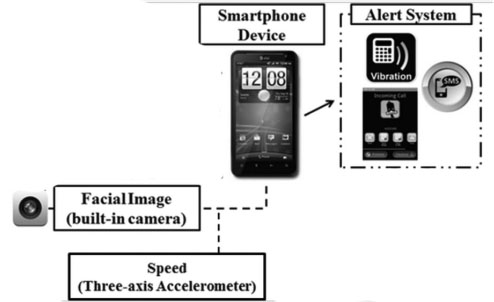
\includegraphics[width= 15cm]{./figures/work.jpg}
    \caption{\label{Fid:1} Working of model}
  
\end{figure}



Eye features, bio signal variation, in-vehicle temperature, and vehicle speed are used to monitor
driver safety level. We propose an Android application solution, our system will collect data from
various sensors such as video, electrocardiography, temperature and a three-axis
accelerometer. If the driver's safety level is compromised then a fake call alerts the driver.
drivers facial image is captured via smartphones front camera.Our application will simply use
computer vision and machine learning algorithms in order to monitor and detect whether the
driver is tired or distracted using the front camera.

\chapter{Feasibility Study}
For the feasibility of this project we conducted an online survey in which we get very positive response
from our target clients. Survey shows that our project having a good market value.
\section{Technical Feasibility}
This system requires a cell phone with high quality camera, navigation system and sensors like
accelerometer etc. The next step is feature extraction from the video which is done by using
Convolutional neural network. For this purpose we have to train a model which requires anaconda
platform, python package and some extra libraries which are used for image classification. All the
required packages and libraries are online available. Model training can be done on CPU system as well
as GPU system with much more faster speed. GPU systems are available in university lab and easily
access able for us.
After this we have to apply image processing techniques on this extracted data and for this
purpose py-torch and torch-vision libraries are used which are also easily access able online.
For the development of android application, we need to install android studio which is online
available and easily download able. The system requirement for android studio at least 8 GB ram with
256 SSD or 500 hard. For the application testing purpose a virtual device can be created or alternatively
a USB cable is required to connect the phone with machine to test the application.
All the required software and machine requirement are easily available which reflects that the
project is technically feasible.

\section{Operational Feasibility}
For the operation of our system it requires a phone with high resolution camera placed on a
fixed place in the car, this camera records the video. A high speed internet is required to transfer the
recorded data from this mobile to the server. When the data is received the trained machine learning
model can categorize the activities of the driver.
The application on the other hand generate the reports on the base of the categorized data by the
trained model. Which is received by the owner of that vehicle.

\section{Economical Feasibility}
Computer machines and smart phones are easily available at low prices these days. For the
development of this project a computer machine and a smart phone is required as a hardware device.
All the other required items are software which are freely available online and easily installed on the
system like anaconda using SPYDER IDE with libraries and android studio for the application
development is also installed on that machine. So, our idea is economically feasible for implementation
in the current scenario.

\chapter{System Requirements}
\section{Hardware Requirements}
As we are are proposing a low budget system for driver behavior analysis so for this we will use
the sensors that are easily available in our android devices. So we will use the following
sensors:
\begin{itemize}
      \item Accelerometer and gyroscope (for speed checking)
    \item GPS (for location identification)
    \item Camera 12 megapixels (for facial expression Detection)
    \item Android Phone
    \item Hard disk minimum 5GB
\end{itemize}
  
    


\section{Software Requirements}
As we are going to develop a mobile application for our system so the software that will be
required for developing our system will b following:
\begin{itemize}
      \item python 3.6
    \item Android Studio
    \item Open CV
    \item pyTorch
    \item tenserflow
    \item Database
\end{itemize}
  
    
\chapter{Limitations and challenges in the implementation of the project}
Beside a lot of advantages and positive impact on our society, there are some limitation of this project.
\begin{itemize}
    \item Privacy Issues \newline
    The first challenge in the implementation of that project is the privacy issue, everybody is not
feeling comfortable for driving in front of camera. Privacy is disturbed due to the video recording of
driver as each and every movement is captured during driving.
\item High Quality Camera \newline
A good camera phone is required for this system, if the camera result is blurred then there is a
possibility that our model can’t detect the correct activity and due to false activity detection false
reports will be generated.
\item High Speed Internet \newline
A high speed internet is required for tracking of location, acceleration measurement and
sending of video data to server for further processing and detection of activity.
\item Camera Location \newline
The recording can be disturbed when the camera phone is used for calling or any other purpose.
Even if the phone is dislocated from the assigned place the activity can’t be monitored accurately.
\end{itemize}

\chapter{References}
\begin{itemize}
    \item J. D. Lee, K. L. Young, M. A. Regon, "Defining driver distraction" in Driver
Distraction: Theory Effects Mitigation, Boca Raton, FL, USA:CRC Press, 2009.
\item W. El Falou, J. Duchêne, M. Grabisch, D. Hewsona, Y. Langerona, and F. Linoc,
“Evaluation of driver discomfort during long-duration car driving,” Applied
Ergonomics, vol. 34, no. 3, pp. 249–255, 2003.
\item The Royal Society for the Prevention of Accidents Driver Fatigue and Road
Accidents: A Literature Review and Position Paper, 2001.
\item IEEE Transactions on Intelligent Transportation Systems ( Volume: 16 , Issue: 6 ,
Dec. 2015)
\item Pakistan Bureau of Statistics,Traffic Accidents(yearly), [pdf]
\item Association for Safe International Road Travel Report on Road Safety Facts and
Annual Global Road Crash Statistics, https://www.asirt.org/safe-travel/road-safety-
facts/
\item Report on Car Accidents in U.S: Facts \& Stats, https://carsurance.net/blog/car-
accident-statistics/
\item Zinebi, K., Souissi, N., \& Tikito, K. (In Press),Driver Behavior Analysis Methods:
Applications oriented study.
\item Zinebi, K., Souissi, N., \& Tikito, K. (In Press) Selecting qualitative features of driver
behavior via Pareto analysis. Transportation Research Part F: Psychology and
Behaviour.
\item Zinebi, K., Souissi, N., \& Tikito, K. (2017, May). Driver behavior quantitative models:
Identification and classification of variables. In Networks, Computers and
Communications (ISNCC), 2017 International Symposium on (pp. 1-6). IEEE.
\end{itemize}




